\documentclass[10pt,conference]{IEEEtran}
% Required by the MSR 2027 Mining Challenge call: IEEEtran conference, no compsoc options, no changes to spacing or
% font size; 4 pages plus 1 page of references; double-anonymous.
\usepackage{cite}
\usepackage{amsmath,amssymb}
\usepackage{graphicx}
\usepackage{booktabs}
\usepackage{xcolor}
\usepackage{url}
\usepackage{tikz}
\usetikzlibrary{arrows.meta,positioning,calc}
\usepackage[hidelinks]{hyperref}
\newcommand{\code}[1]{\texttt{\small #1}}  % used in the co-author sections

% Placeholders. Every \cn{} and \todo{} must be gone before submission (grep for them).
\newcommand{\cn}[1]{\textcolor{red}{[CITE: #1]}}
\newcommand{\todo}[1]{\textcolor{blue}{[#1]}}

\begin{document}

\title{\todo{Title: proposal P1 in the brief}}
\author{\IEEEauthorblockN{Anonymous Author(s)}}
\maketitle

\begin{abstract}
\todo{Abstract, written last. Must state the dataset version: GitSkills, July 2026 snapshot (arXiv 2608.10906 v3;
Zenodo 10.5281/zenodo.21875637).}
\end{abstract}

\begin{IEEEkeywords}
\todo{Keywords}
\end{IEEEkeywords}

% Co-author text, unchanged. Proposals P2 (reframe) and P8 in the brief are not applied.
\section{Introduction}
\label{sec:introduction}

Skills are small instruction files that extend coding agents~\cite{anthropicskillsblog}. Each skill carries a name and a short description. When the user asks for something, the agent reads the list of names and descriptions and decides which skill, if any, to load. The main products all select skills this way, and none of them checks whether two entries in the list say the same thing~\cite{claudecodeskills,codexskills,agentskillsspec}. Claude Code's documentation acknowledges the risk: when descriptions are vague or overlap, the agent may load the wrong skill or miss a useful one~\cite{claudecodeskills}.

Skills are also copied heavily. In GitSkills~\cite{gitskills}, half of all occurrences are byte-for-byte copies of a file in another repository, and a tenth of repositories keep parallel copies for several agents. Software engineering research has long documented what happens to copied code: copies drift, and a fix lands in one copy but not the others~\cite{kim2005genealogies,juergens2009clones}. We expect the same with skills, with one difference. The reader of a stale copy is a language model, not a developer who might notice that something looks out of date.

We study two ways a skill list can go wrong. A \emph{conflicting copy} is the same skill name in two agent directories of one repository with different content, so that, for example, Claude Code and Codex read different instructions under one name. \emph{Competing skills} are two differently named skills in one catalog whose descriptions overlap so much that a realistic request could reasonably go to either. Recent experimental work shows that competition lowers selection accuracy~\cite{li2026singleagent,chen2026scaling,song2026shadowing,yan2026oneskill}, but no study has measured drift between mirrored copies, and the prevalence of competition has not been measured on GitSkills or with human labels and a sampling design. We ask:

\begin{itemize}
\item \textbf{RQ1 (conflicting copies).} How often does a repository give its coding agents different copies of the same skill?
\item \textbf{RQ2 (competing skills).} How often do differently named skills in one catalog compete?
\item \textbf{RQ3 (author practices).} What do skill authors do to prevent either problem?
\end{itemize}

Our contributions are (1) exact counts of conflicting copies across all eligible repositories, broken down by which product reads which directory; (2) a codebook for competing skills and a reliability study on 180 human-labeled pairs that shows where coders disagree; and (3) counts of cross-references, negative triggers and invocation flags that show how authors guard against overlap.


% Co-author text, unchanged. Proposal P4 (trim to about 0.45 page) is not applied.
\section{Background and Related Work}
\label{sec:background}

\textbf{How agents select skills.} A skill is a folder with a SKILL.md file whose YAML front matter holds at least a name and a description~\cite{agentskillsspec}. At the start of a session the agent shows the model only the names and descriptions; the full text is loaded when the model picks a skill. A skill with \code{disable-model-invocation: true} is never shown to the model~\cite{claudecodeskills}. Each product reads its own directories. As documented in July 2026, Claude Code reads \code{.claude/skills} and Codex reads \code{.agents/skills}, while Copilot and Cursor read several directories at once~\cite{claudecodeskills,codexskills,vscodeskills,cursorskills} (Table~\ref{tab:dirs}). When two skills share a name, Claude Code prefers a personal skill over a project skill, and Codex lists both; the user is not told when either rule applies.

\textbf{Skill selection under competition.} Choosing among similar options is a known problem for tool-using LLMs~\cite{huang2024metatool,qin2024toolllm}. For skills, adding one near-synonym competitor per skill cut selection accuracy by 7 to 30\%, and two by 17 to 63\%~\cite{li2026singleagent}. Routing accuracy falls with the logarithm of library size across 15 models, and errors start as competition between closely related skills~\cite{chen2026scaling}. Pass rates fell by up to 21\% at 202 skills because of wrong selection, not longer context~\cite{song2026shadowing}. A production team named the problem ``skill collision'' and found that rewriting descriptions cannot separate skills whose intended scopes overlap~\cite{zhou2026single}. When two same-job skills are loaded together, one usually takes over: rule-following drops from 93 to 99\% to 61 to 62\% across seven models~\cite{razmara2026takeover}.

\textbf{Closest work.} Yan et al.~\cite{yan2026oneskill} mined 105,302 skill copies in 20,947 repositories, reconstructed 5,106 installation lists, and judged similar pairs with embeddings and an LLM. Nearly one in four installed skills had a similar co-installed skill, and in 6,368 Claude Code runs the installed skill was used 19.9 percentage points less often when one was present. Their inventory excludes other agents' directories and does not examine drift between copies.

\textbf{Skills and agent configuration as artifacts.} Skills are one of eight repository-level mechanisms for configuring coding agents~\cite{galster2026configuring}. Context files such as AGENTS.md evolve like configuration code~\cite{chatlatanagulchai2025readmes,mohsenimofidi2026context}, often contain smells~\cite{dossantos2026smells}, and have mixed effects on agents~\cite{gloaguen2026agentsmd,lulla2026impact}. Most SKILL.md files contain at least one quality defect~\cite{hong2026smells,zhang2026reusable}. These studies look at defects within one file; we look at defects that appear only between two.

\textbf{Code cloning and copy-based reuse.} Most files on GitHub have a duplicate: only 85 million of 482 million files in 4.5 million non-fork projects are unique~\cite{lopes2017dejavu}. Clones evolve independently~\cite{kim2005genealogies}, inconsistent changes to clones are a common source of faults~\cite{juergens2009clones}, and some copies are deliberate adaptations~\cite{kapser2008cloning}. Copying from outside sources is common and often unattributed~\cite{baltes2019snippets}. For skills, 53\% of reused skills are never modified after adoption~\cite{gao2026registry}, and 67.3\% of Cursor rules files are never changed after creation~\cite{sun2026cursorrules}. Skill clones are widespread across authors~\cite{zhu2026latent}, and 58.7\% of skills share a name with another skill~\cite{jia2026islands}. We apply the clone-drift lens to a new case: copies of one skill kept in parallel for different agents.


% Co-author section heading, subsection A, Table I and Fig. 1, unchanged (proposal P6 not applied).
\section{Data and Method}
\label{sec:data_method}

\subsection{GitSkills and catalogs}

GitSkills~\cite{gitskills} was mined from public GitHub repositories between July 9 and July 20, 2026. Its artifacts table has 3,797,117 SKILL.md occurrences (repository plus path), which collapse to 1,877,981 distinct contents. One copy per content carries the text, front matter and commit history, so we join the table to itself on \code{file\_sha}. We use the Hugging Face Parquet export, processed one part at a time with DuckDB, and July 20, 2026 as the reference date.

A skill is \emph{valid} if the file is named exactly SKILL.md and its front matter parses with a non-empty name and description (89.2\% of occurrences). A \emph{catalog} is the set of valid skills in one repository under one agent directory at the repository root (\code{.<agent>/skills/<folder>/SKILL.md}). This gives 141,458 catalogs in 120,929 repositories (Fig.~\ref{fig:design}). We key skills on the front-matter name, trimmed and lower-cased, because that is what products display; it differs from the folder name in 24.3\% of valid occurrences.

\begin{table}[t]
\centering
\caption{Catalogs by agent directory and the products that read them (July 2026 documentation).}
\label{tab:dirs}
\footnotesize
\setlength{\tabcolsep}{4pt}
\begin{tabular}{lrccccc}
\toprule
Directory & Catalogs & Claude & Codex & Copilot & Cursor & OpenCode \\
\midrule
\code{.claude}  & 57,523 & \checkmark &            & \checkmark & \checkmark & \checkmark \\
\code{.agents}  & 36,838 &            & \checkmark & \checkmark & \checkmark & \checkmark \\
\code{.github}  & 12,918 &            &            & \checkmark &            &            \\
\code{.cursor}  &  7,125 &            &            &            & \checkmark &            \\
\code{.codex}   &  5,195 &            &            &            & \checkmark &            \\
Other           & 21,859 &            &            &            &            &            \\
\midrule
Total           & 141,458 & & & & & \\
\bottomrule
\end{tabular}
\end{table}

\begin{figure}[t]
\centering
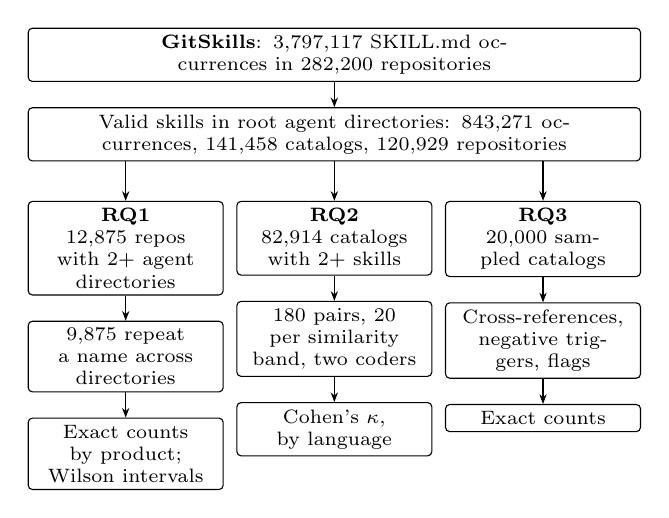
\begin{tikzpicture}[
  font=\scriptsize,
  box/.style={draw, rounded corners=1.5pt, align=center, inner sep=2.5pt, fill=white},
  arr/.style={-{Stealth[length=3.5pt]}, thin},
  node distance=3.2mm]
\node[box, text width=7.6cm] (all) {\textbf{GitSkills}: 3,797,117 SKILL.md occurrences in 282,200 repositories};
\node[box, text width=7.6cm, below=of all] (valid) {Valid skills in root agent directories: 843,271 occurrences, 141,458 catalogs, 120,929 repositories};
\node[box, text width=2.3cm, below=5mm of valid.south west, anchor=north west] (r1a) {\textbf{RQ1}\\12,875 repos with 2+ agent directories};
\node[box, text width=2.3cm, below=5mm of valid.south, anchor=north] (r2a) {\textbf{RQ2}\\82,914 catalogs with 2+ skills};
\node[box, text width=2.3cm, below=5mm of valid.south east, anchor=north east] (r3a) {\textbf{RQ3}\\20,000 sampled catalogs};
\node[box, text width=2.3cm, below=of r1a] (r1b) {9,875 repeat a name across directories};
\node[box, text width=2.3cm, below=of r2a] (r2b) {180 pairs, 20 per similarity band, two coders};
\node[box, text width=2.3cm, below=of r3a] (r3b) {Cross-references, negative triggers, flags};
\node[box, text width=2.3cm, below=of r1b] (r1c) {Exact counts by product; Wilson intervals};
\node[box, text width=2.3cm, below=of r2b] (r2c) {Cohen's $\kappa$, by language};
\node[box, text width=2.3cm, below=of r3b] (r3c) {Exact counts};
\draw[arr] (all) -- (valid);
\draw[arr] (valid.south -| r1a) -- (r1a);
\draw[arr] (valid) -- (r2a);
\draw[arr] (valid.south -| r3a) -- (r3a);
\foreach \a/\b in {r1a/r1b, r1b/r1c, r2a/r2b, r2b/r2c, r3a/r3b, r3b/r3c} \draw[arr] (\a) -- (\b);
\end{tikzpicture}
\caption{Study design. RQ1 is an exact count over all eligible repositories; RQ2 is a human-labeled sample; RQ3 is counted on a sample of 20,000 catalogs.}
\label{fig:design}
\end{figure}


% Proposal P3, applied provisionally: the drafted subsections replace the co-author's RQ1 subsection.
% To restore hers, swap the two lines below.
% \subsection{RQ1: Conflicting copies}

The RQ1 population is the 12,875 repositories with valid skills in two or more root agent directories; 9,875 of them repeat at least one name across directories. A copy is \emph{diverged} when the same name appears in two directories of one repository with different \code{file\_sha} values. For each diverged name we record whether the description differs and whether the body length differs by more than 5\% and 50 characters. A different hash is an upper bound on meaningful change, since line endings, whitespace and agent-specific syntax (for example \code{/prp-debug} against \code{\$prp-debug}) also change it. We report counts by the directories each product reads, since one repository can present a conflict to Copilot or Cursor but not to Claude Code, and give Wilson 95\% intervals for every rate~\cite{wilson1927}.


% Data and method, subsections B and C. Drafted 2026-11-18 from docs/runlog.md (entries of 2026-11-17 and 2026-11-18).
% Replaces subsection B ("RQ1: Conflicting copies") of the co-author draft; see the brief, proposal P3.

\subsection{Measuring each repository at the snapshot}
\label{sec:sample}

To see what the dataset misses, we compared it with the repositories it was mined from, as they stood when it was
mined. The frame was every non-fork repository with a valid skill under a root agent directory
(P1, 120,926 repositories). We split P1 into four strata by what the dataset shows for each repository: project
repositories (P2, defined below) with one agent directory and one skill name (46,715), with one agent directory and
two or more names (48,746), with two or more agent directories (9,721), and repositories outside P2 (15,744). We
drew 400, 800, 800 and 300 repositories from these strata by simple random sampling (2,300 in all; seed 20261008).
P2 excludes skill collections: repositories whose name or description matches a list of collection keywords, whose
number of distinct skill names lies above the Tukey upper fence of the per-repository distribution, or that have no
detected language, no skill in \texttt{.claude/skills} and two or more skills. The keyword list and the fence follow Gao et al.~\cite{gao2026registry}; the language rule is ours. P3, used only as a check, further reduces each group of
near-forks and templates in P2 to one repository (identical sets of skill hashes, or a Jaccard similarity of at least
0.8 with five or more shared hashes).

For each sampled repository we took the last commit on the default branch before the end of the dataset's mining
window (2026-07-20 22:26 UTC) and read the recursive tree at that commit through the GitHub REST API. The tree gives
every \texttt{SKILL.md} path with its git blob SHA, which is the hash GitSkills stores as \texttt{file\_sha}. We
count \emph{root skill files}, paths of the form \texttt{.<agent>/skills/<folder>/SKILL.md}, whose
\emph{agent directory} is \texttt{.<agent>}. A repository can change while the search is still running, so for the 672 repositories whose snapshot commit fell
inside the window (after 2026-07-09 17:26 UTC) we also read the tree at the start of the window. A root skill file counts as
present throughout when its path is in the tree at both ends. We compared these files with every dataset row for the
repository, valid or not, matching on path. A file the dataset lacks is an \emph{identical copy} when its blob SHA
equals a \texttt{file\_sha} the dataset holds for the same repository, and \emph{missing content} otherwise.
Coverage is the share of present files that the dataset holds, and a repository is \emph{complete} when the
dataset holds all of them.

Of the 2,300 repositories, 217 were deleted, private or had no commit before the snapshot (8 to 10\% in every
stratum) and were dropped. The remaining repositories in each stratum carry its weight (stratum size over
repositories available).
Two trees were truncated by the API and are kept. We report weighted ratio estimates with 95\% percentile intervals
from 2,000 bootstrap replicates drawn within strata. The design was fixed in our run log before the sample was drawn,
and the estimation script was written and tested on synthetic data before its first run.

\subsection{RQ1: Mirrored and diverged skills, measured twice}
\label{sec:rq1method}

Each sampled repository in P2 was measured twice with the same rules: once from its tree at the snapshot and once
from its dataset rows. Because a tree lists paths but not file contents, we name a skill by its folder,
lower-cased, on both sides. A \emph{mirrored} name appears in two or more agent directories of one repository; it is
\emph{diverged} when its copies have two or more distinct blob SHAs. A different hash is an upper bound on meaningful
change, since line endings, whitespace and agent-specific syntax also change it. We estimate the share of
repositories with two or more agent directories, the share with a mirrored name, the share of those with a diverged
name, and the share of mirrored names that are diverged, each from both versions, with the paired difference
(tree minus dataset) computed within every bootstrap replicate.

\subsection{RQ2: Competing skills}

Two skills compete when a realistic request exists for which an agent reading only their names and descriptions could reasonably pick either. Our codebook also assigns a relation type: D (duplicate or variant), S (one scope contains the other) or O (partial overlap). The population is the 82,914 catalogs with two or more skills, excluding skills closed to model invocation (2.45\% of skills). Coders see the name and description in original case, cut at the 1,536-character product cap.

We stratify candidate pairs by the cosine similarity of description embeddings (all-MiniLM-L6-v2~\cite{reimers2019sbert}) and draw 20 pairs per similarity band, 180 in all. Similarity only decides which pairs are read; it does not identify competition, since in an earlier pilot no similarity band reached 80\% competing pairs.

\textbf{Reliability.} Both coders labeled the 180 pairs independently. We set a threshold of Cohen's $\kappa$~\cite{cohen1960kappa} of 0.60 on competing versus not competing, the top of the ``moderate'' band~\cite{landis1977kappa}, before labeling. An LLM given only the codebook labeled the same pairs as a third reader, for comparison only. Because 29 of the 180 pairs (16\%) are not in English, both coders used one shared DeepL translation, and we report $\kappa$ separately for English and translated pairs.


% Proposal P5, applied provisionally: RQ3 is left out for space. To restore, uncomment.
% \subsection{RQ3: Author practices}

On a random sample of 20,000 catalogs (192,422 skills) we count descriptions that name another skill in the same catalog (hyphenated names, as whole tokens), descriptions with negative-trigger wording (``do not use'', ``not for'', ``not intended for'' and similar), and front-matter invocation flags. All patterns were fixed in our run log before counting. A first rule that matched any name of six or more characters was inflated by names that are ordinary words, so we match hyphenated names only; the change is logged. The invocation flag is counted over all valid skills.


\section{Results}
% Results, subsections A and B. Drafted 2026-11-18. Every number is in data/private/rq1/estimates.csv or the
% run-log entries of 2026-11-04 to 2026-11-18; see the claim-evidence map in paper-brief.md.

\subsection{The dataset holds about half the skill files of project repositories}
\label{sec:coverage}

In project repositories, GitSkills holds 54.2\% of the root skill files that were present throughout the mining
window (95\% CI 51.2 to 57.5; Table~\ref{tab:estimates}), and half of these repositories (49.9\%) are complete.
Across all repositories the estimate is 62.6\% (54.0 to 67.7). That interval is wide and lopsided because five very
large repositories outside P2 carry 44\% of the weighted files; the project-repository figure does not depend on
them. The loss is not confined to large repositories: in the sample, repositories that the dataset shows with a
single skill hold 905 root skill files present throughout, of which the dataset has 424.

The missing files are mostly content the dataset does not hold. Identical copies of a file the dataset already has
for the same repository make up 7.0\% of missing files in project repositories (5.2 to 9.3) and 10.1\% overall
(4.0 to 20.2). A rule that dropped repeated files would remove only identical copies, so it cannot account for most of
the gap.

\subsection{Why files are missing}
\label{sec:cause}

Code search returns at most 1,000 results per query~\cite{github-search}, so GitSkills partitioned its search by file
size and split any size range that returned more than 1,000 results~\cite{gitskills}. A range one byte wide cannot be
split further. On 2026-11-17 the query \texttt{filename:SKILL.md size:3140..3140} reported 1,910 results; page~10
returned 100 items and page~11 was refused with HTTP~422 (``Cannot access beyond the first 1000 results''). Every file
past the first 1,000 in such a bucket is unreachable, whether it is unique or a copy: a query restricted to one
repository returned all four of its \texttt{SKILL.md} files, three of them byte-identical. In that test the search did
not merge copies. The dataset's authors also report that the search's \texttt{total\_count} was unreliable, which
can hide a full bucket~\cite{gitskills}. We cannot replay the July search, and the index has grown since (code search
reported 8.0 million \texttt{SKILL.md} files on 2026-11-17, against 3.8 million retrieved in July), so the
demonstration shows the mechanism, not the July bucket sizes.

\begin{table}[t]
\centering
\caption{Estimates from 2,083 repositories measured at the snapshot (percent, 95\% bootstrap interval)}
\label{tab:estimates}
\footnotesize
\setlength{\tabcolsep}{2.5pt}
\begin{tabular*}{\columnwidth}{@{\extracolsep{\fill}}lrrr@{}}
\toprule
\textit{Coverage, files present throughout} & \multicolumn{2}{r}{P2 (projects)} & P1 (all) \\
\midrule
Files held by the dataset & \multicolumn{2}{r}{54.2 (51.2--57.5)} & 62.6 (54.0--67.7) \\
Repositories complete & \multicolumn{2}{r}{49.9 (47.3--52.7)} & 46.3 (43.8--48.8) \\
Missing files that are identical copies & \multicolumn{2}{r}{7.0 (5.2--9.3)} & 10.1 (4.0--20.2) \\
\midrule
\textit{RQ1, project repositories (P2)} & Tree & Dataset & Difference \\
\midrule
Two or more agent directories & 14.7 & 9.4 & $+$5.3 (3.9--6.7) \\
A mirrored name & 11.0 & 7.0 & $+$4.0 (2.9--5.2) \\
\quad of those, a diverged name & 38.1 & 32.3 & $+$5.8 (0.4--11.8) \\
Mirrored names that diverged & 23.5 & 24.7 & $-$1.2 ($-$5.9--3.3) \\
\bottomrule
\end{tabular*}
\end{table}

\subsection{RQ1: The dataset undercounts mirroring but not its drift rate}
\label{sec:rq1}

Measured from the trees, 11.0\% of project repositories keep the same skill name in two or more agent directories;
38.1\% of those hold at least one diverged copy, and 23.5\% of mirrored names have diverged (Table~\ref{tab:estimates}).
Measured from the dataset, the same repositories look less mirrored: 9.4\% instead of 14.7\% have two or more agent
directories, and 7.0\% instead of 11.0\% have a mirrored name, so the dataset misses about a third of mirroring
repositories. The share of mirrored names that diverge is about the same from both (23.5\% against 24.7\%, difference $-1.2$
points, $-5.9$ to 3.3). Per repository, the share with a diverged copy is somewhat higher from the trees ($+5.8$
points, 0.4 to 11.8), which is consistent with the trees showing more mirrored names per repository, and so more
chances for one of them to diverge. Restricting to P3, where near-forks and templates are collapsed, moves every
difference in the same direction, and dropping the two truncated trees changes no estimate by more than 0.1 points.

\subsection{RQ2: Competing skills}
\todo{RESULT NEEDED: RQ2 on about 300 pairs, if run.}

\section{Discussion}
\todo{Answer to the opening question; implications for users of the dataset (use per-name rates, re-measure
prevalence from trees, or apply the repair); limitations: root agent directories and the default branch only,
repositories the search never returned are not measured, folder names stand in for front-matter names, 8 to 10\% of
sampled repositories unavailable.}

\section{Ethics}
% Policy section: the authors write it. Facts available: public repositories only; no personal data stored or
% reported; repository names stay out of the paper and the package; results are aggregates; the dataset's authors
% will receive the reproduction and repair after review.
\todo{AUTHOR: ethics section (required by the call, before the conclusion).}

\section{Conclusion}
\todo{Conclusion.}

\section*{Acknowledgment}
\todo{AUTHOR: IEEE disclosure of AI-generated content, from the AI-use log in the brief.}

\bibliographystyle{IEEEtran}
\bibliography{references}
\end{document}
